\documentclass[12pt]{article}
\usepackage[utf8]{inputenc}
\usepackage{graphicx}

\begin{document}

\title{Comparison of K-point selection methods.}

\author{Wiley Morgan, Gus L. W. Hart}
%% \affiliation
%% {Department of Physics and Astronomy, Brigham Young University, Provo Utah 84602 USA}

%% \author{Gus Hart}
%% \affiliation
%% {Department of Physics and Astronomy Brigham Young University, Provo Utah 84602 USA}

\date{May 2016}

\maketitle

\section*{Description of plot}

The plot displayed in Fig. \ref{fig:all_vs_Mueller} is a
representation of the ``speed-up'' that the Mueller K-point method
offers over the Froyen method and the methods employed by AFLOW. By
speed-up we mean the ratio of the irreducible K-points used by either
the Froyen or AFLOW method to the Mueller method (i.e., Froyen or
AFLOW/Mueller irreducible K-points). The data was generated from three
systems; pure Co, pure W, and pure V with cell sizes ranging from 1 to
11 atoms per cell for each system. The tests were also run over
different K-point densities ranging from 1 to $22^3$ K-points per
reciprocal atom The K-points used for each method were generated as
follows, for the Froyen method only K-point density that were
commensurate with the cell size were used. The K-point grids for the
Froyen method were generated by dividing the number cubed root of
K-points per reciprocal atom by each lattice vector to create a
uniform K-point grid for each cell and K-point density. The K-points
grids for AFLOW were generated by putting the desired number of
K-points per reciprocal atom into the correct location in the AFLOW
aflow.in script, AFLOW was then allowed to generate the K-points using
whichever methods it would use by default. For the Mueller method
$r\_min$ was found using the following equation:

\begin{equation}
  r\_min ~= 2.8074(k_n^{1/3})-3.4008
\end{equation}

where $k_n$ is the number of K-points per reciprocal atom. The
database of Mueller K-point grids was then queried for a system with
the desired $r\_min$ and a KPOINTS file generated. The program VASP
was used to calculate the energy of each system for each cell size and
K-point density available to determine the energy of the systems.

Once all VASP calculations were complete, for the Froyen and Mueller
methods only 20 NSW steps were permitted however the default value of
NSW=52 for AFLOW could not be overwritten so the AFLOW tests used more
ionic steps in some cases, the resulting energies were divided by the
number of atoms in the cell in order to easily compare the values. The
converged energy was then taken to be the energy of the largest system
with the highest K-point density. The difference between each systems
energy per atom and the converged energy per atom was taken as a
measure of the accuracy of the calculation, i.e., the systems error.

In order to generate Fig. \ref{fig:all_vs_Mueller} the range of the
errors, roughly $10^{-6}$ to $10^2$, was discretized into steps of
size 0.001 on a log scale ($10^x$ with $-6<=x<=2$) to make an discrete
error space. For each point in this error space the K-point methods
were searched for the largest error that was $>=$ to the point (this
was done for each system Co, W, and V and each cell size
separately). Once the K-point density whose error meant these
conditions was found for each method the ratio of the Froyen and
Mueller irreducible K-points and the ration of the ALFOW and Mueller
irreducible K-points were found and saved for that error value. This
process produced 33 different speed-up data sets for each method
comparison. Fig. \ref{fig:all_vs_Mueller} shows the results of averaging
those 33 data sets by adding together all the runs at each error and
dividing by the number of runs.

The plot itself shows that, on average, the Mueller method is always
better than the Froyen method by nearly a factor of 10. The comparison
with the AFLOW method shows that, on average, the Mueller method can
be faster except when accuracies smaller than $10^{-5}$ are
desired\footnote{The fact that AFLOW outperformed the Mueller method
  in the small error region could partially be explained by the fact
  the AFLOW runs didn't converge to the same energy for the different
  cell sizes. As a result only a few of the AFLOW runs achieved
  accuracy to this level while most of the Mueller and Froyen runs
  reached the small error region.}.

\begin{figure*}
  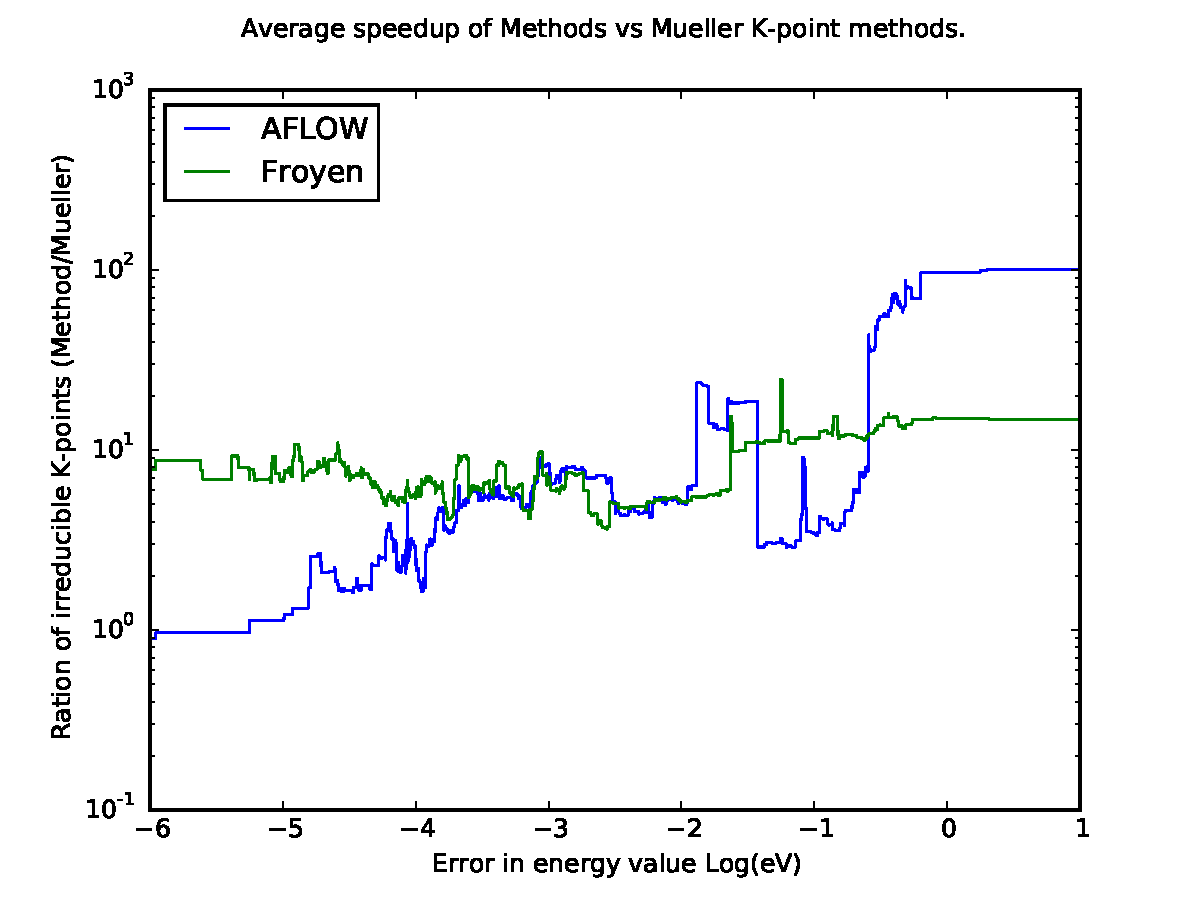
\includegraphics[scale=0.75]{All_vs_Mueller.pdf}
  \caption{The ratio of irreducible K-points vs error in calculated
    energy for each method vs the Mueller method. Both axis are on log scales.}
  \label{fig:all_vs_Mueller}
\end{figure*}

\end{document}
